\section{Parallel coordinate descent methods}\label{pcdm}
In this section, we introduce the parallel coordinate descent algorithm, which benefits significantly from our $PSF$ approximation scheme. The $PSF$ approximation we developed lets the deconvolution algorithm use an approximate $PSF$. It uses only the center window of the full $PSF$, where each side of the window is a fraction of the full $PSF$. Or in other words: The approximation method resulted in a sparse $PSF$ for the deconvolution algorithm. We use the introduced sparsity for parallel deconvolutions, resulting in the parallel coordinate descent algorithm

The serial coordinate descent algorithm minimizes a single pixel in each iteration. Parallel coordinate descent methods can group several pixels into blocks, and minimize multiple blocks in parallel within a single iteration. 

T

We introduce the new concepts of the parallel methods in Section \ref{pcdm:pcdm}, and show synchronous implementations of the new parallel coordinate descent algorithm. We then show an efficient, and asynchronous implementation of our parallel algorithm in Section \ref{pcdm:async}, where each processor updates a block independently of the other processors.


The parallel coordinate descent algorithm from Section \ref{pcdm:async} does not run efficiently on the deconvolution problem. We discuss the problems and our extensions we developed for an efficient parallel coordinate descent deconvolution algorithm in Section \ref{pcdm:adaption}.


\subsection{From serial to parallel coordinate descent}\label{pcdm:pcdm}
We start with our serial coordinate descent algorithm and first modify it to a serial block coordinate descent algorithm. A block is a group of pixels. In our case, a block is always a rectangle of neighboring pixels. For example: A block of $4^2$ pixels can be minimized in a single iteration of the serial block coordinate descent algorithm.

Later in Section \ref{pcdm:pcdm:eso} we introduce the main concept which allows us to adapt the serial block algorithm to a parallel block coordinate descent algorithm. We show a synchronous implementation of the parallel coordinate descent algorithm in Section \ref{pcdm:pcdm:approx}.



\subsubsection{Estimated Separability Overapproximation (ESO)} \label{pcdm:pcdm:eso}
So far, we introduced a serial block coordinate descent algorithm. If we want to update blocks of pixels in parallel, we need to estimate how much the $PSF$s of parallel updates 'overlap'. For example: If we update two blocks in parallel, and their combined $PSF$s do not overlap, then the update is independent. Updating the first block, and then the second block in a serial algorithm leads to the same result as updating both blocks in parallel. 

However, if we update two blocks, which are located next to each other in the image, then their combined $PSF$s overlap significantly. Their updates are dependent on each other. If we update the first block, and then the second block in a serial algorithm results in significantly lower pixel values for the second block. Because their $PSF$s overlap, both blocks try to explain mostly the same emission. If we update both blocks in parallel, each block would try to explain the same emission, and we would over-estimate their pixel values.

This over-estimation can lead to a diverging algorithm. To guarantee the convergence of a parallel block coordinate descent, we need to estimate the overlap of the $PSF$s of parallel updates. This can be done with the Estimated Separability Overapproximation (ESO) developed in \cite{richtarik2016parallel}. The ESO estimates how much the $PSF$s overlap, if we update $\tau$ random blocks in parallel:

\begin{equation}\label{pcdm:pcdm:eso}
ESO(\omega, \tau, n) = 1+ \frac{(\omega - 1)(\tau - 1)}{max(1, n -1)}
\end{equation}

Where $\omega$ is the number of non-zero entries in the $PSF$, $\tau$ is the number of random parallel updates in each iteration, and $n$ is the number of blocks in the image. Let us use an example to demonstrate what the ESO means: Let us assume the $PSF$ has $\omega = 24$ non zero entries, $\tau = 4$ processors to update in parallel, and the image is $256^2$ pixels in size with a block size of $4^2$ pixels. Plugging the values into the ESO gives us the following result:

\begin{equation}
ESO(\omega = 24, \tau = 4, n = (256^2 / 4^2)) = 1+ \frac{(24 - 1)(4 - 1)}{max(1, 4096 -1)} \approx 1.017
\end{equation}

An ESO of $1$ means the $\tau = 4$ parallel updates are completely independent of each other, and we do not need to account for overlapping $PSF$s. In our example, we arrived at an ESO of $1.017$. This means every parallel update step has to be divided by $1.017$ to account for overlapping $PSF$s, and ensure convergence.

The ESO only needs to know the number of non-zero components. It is independent of the exact structure of the $PSF$. The fewer non-zero components the $PSF$ has, the closer it is to 1, and the more effective each parallel update is. The ESO benefits from our $PSF$ approximation. It decreases the number of non-zero components in the $PSF$ and leads to an ESO closer to 1.

However, note that the ESO assumes we choose $\tau = 4$ blocks uniformly at random. Indeed, a uniform random selection strategy is a core assumption for the parallel coordinate descent method\cite{richtarik2016parallel}. Random selection strategies tend to perform badly on the deconvolution problem. Later in Section \ref{pcdm:adaption}, we develop a pseudo-random selection strategy which does not break the random selection assumption of the ESO, but performs better on the deconvolution problem.


\subsubsection{Accelerated parallel block coordinate descent} \label{pcdm:pcdm:approx}
So far, we introduced the serial block coordinate descent and the ESO. The serial block coordinate descent can update a block of pixels in a single iteration, and the ESO estimates how much $PSF$s overlap when we perform parallel update steps. In this section, we put this together in an accelerated, parallel block coordinate descent algorithm based on APPROX\cite{fercoq2015accelerated}. But first, we introduce gradient acceleration.

In gradient acceleration, we use the gradient from previous iterations to speed up convergence of the current iteration. We can accelerate our serial coordinate descent algorithm by extending it with an acceleration parameter $\theta$, a copy of the gradient map and a copy of the reconstructed image $x$.  We term one couple of gradient map plus reconstructed image as 'explore', while the other couple is called 'correction'. The 'correction' gradient map and reconstructed image contain gradient information of the previous iterations. They are used to speed up the convergence of the 'explore'. In each iteration, the acceleration parameter $\theta$ decreases, and we use more information from the 'correction' gradient map and reconstruction.

This leads to the following accelerated, parallel and block coordinate descent deconvolution algorithm:
\begin{lstlisting}
dirty = IFFT(GridVisibilities(visibilities))
residualsPadded = ZeroPadding(dirty)

psfPadded = ZeroPadding(PSF)
psfPadded = FlipUD(FlipLR(psfPadded))
gradientUpdate = iFFT(FFT(ZeroPadding(PSF)) * FFT(psfPadded))

xExplore = new Array[,]
xCorrection = new Array[,]
gradientsMapExplore = iFFT(FFT(residualsPadded) * FFT(psfPadded))
gradientMapCorrection = new Array[,]
lipschitzMap = CalcLipschitz(PSF)

eso = ESO(CountNonZero(PSF), t, x.Length / blockSize)
theta0 = t / (x.Length / blockSize)
theta = theta0

do 
	oldObjectiveValue = objectiveValue
	
	//Step 1: select t blocks uniformly at random
	blocks = sample(t)
	
	//Step 2: update reconstruction in parallel
	diffBlocks = new Array
	parallel for each block in blocks
		//increase blockLipschitz according to the ESO
		blockLipschitz = Sum(GetBlock(LipschitzMap, block))
		blockLipschitz = blockLipschitz * eso
		
		oldBlock = GetBlock(xExplore, block)
		tmp = theta^2 * GetBlock(gradientsMapCorrection, block) 
			+ GetBlock(gradientsMapExplore, block) 
			+ GetBLock(xExplore, block) * blockLipschitz
		optimalBlock = Max(tmp - lambda*alpha) / (blockLipschitz + (1 - alpha)*lambda)
		diffBlock = optimalBlock - oldBlock
		
		xExplore[block] += diffBlock
		xCorrection[block] += diffBlock * (-(1.0f - theta / theta0) / theta^2)
		diffBlocks[block] = diffBlock
	
	//Step 3: Update gradients
	for each block in blocks
		diffBlock = diffBlocks[block]
		for each pixel in block
			diff = diffBlock[pixel]
			shiftedUpdate = Shift(gradientUpdate, pixelLocation)
			
			gradientsMapExplore = gradientsMapExplore - shiftedUpdate * diff
			gradientsMapCorrection = gradientsMapCorrection - shiftedUpdate * diff * (-(1.0f - theta / theta0) / theta^2)
	
	theta = (Sqrt((theta^2 * theta^2) + 4 * (theta^2)) - theta^2) / 2.0f
while maxAbsDiff  < epsilon

output = new float[,]
for(i in in Range(0, dirty.Length(0))
	for(j in in Range(0, dirty.Length(0))
		output[i, j] = theta * xCorrection[i, j] + xExplore[i, j];
\end{lstlisting}

In each iteration, the parallel algorithm first samples $\tau$ unique blocks uniformly at random (we cannot select the same block more than in a single iteration). In the second step, we then update each block in parallel. Note that we multiply the block Lipschitz constant with the ESO, which ensures convergence for parallel updates. In the third step, we update the two gradient maps. The final image is a combination of the two reconstructed images $x$ from the 'explore' and 'correction' couple.

This algorithm is parallel, but it is still synchronized: It updates each block in parallel, but waits for all updates to finish before continuing with the next iteration. In the next Section \ref{pcdm:async}, we introduce an asynchronous implementation, where the individual processors do not wait for each other.

The accelerated, parallel coordinate descent algorithm reduces itself to a non-accelerated variant, if we do not modify $\theta$ in each iteration. In that case, the 'correction' gradient map and reconstruction $x$ stay zero over the course of the algorithm. Note that due to gradient acceleration, we need twice the memory (for the 'correction' maps), and twice the number of operations to update a single block. Gradient acceleration allows us to take larger steps towards the optimum in each iteration. As such, it should need fewer iterations to converge than the non-accelerated variant. But a single iteration of the accelerated variant is more expensive.


\subsection{Asynchronous implementation}\label{pcdm:async}
In this section, we show how the accelerated, parallel coordinate descent algorithm can be implemented asynchronously. Each processor selects a random block, and updates the gradient maps and reconstructed images independently of the other processors. The asynchronous processors have to communicate three parts: The 'explore' gradient map, the 'correction' gradient map, and what block they have currently selected to update.

For the asynchronous implementation, we introduce the 'blockLocks' map. Each asynchronous processor writes its processor id at the location of the block it is currently updating. A processor can only select a block which is not updated by another processor. The write to the blockLocks map has to be atomic, such as the updates on the 'explore' and 'correction' gradient map. This leads to the following algorithM:


\begin{lstlisting}
...
concurrentIterations = 1000
blockLocks = new Array[,]
...
do
	//asynchronous iterations
	parallelDiffs = new Array[]
	parallel for each processorId in (0:t)+1
		for concurrentIter in 0:concurrentIterations
			block = AtomicLockRandomBlock(blockLocks, processorId)
			
			...		
			//Step 2: update block according to the same update rule
			...
			
			parallelDiffs[processorId -1] = Max(parallelDiffs[processorId -1], diffBlock)
			
			//Step 3: Update gradients
			for each pixel in block
				diff = diffBlock[pixel]
				shiftedUpdate = Shift(gradientUpdate, pixelLocation)
				
				AtomicSum(gradientsMapExplore, -shiftedUpdate * diff)
				AtomicSum(gradientsMapCorrection, -shiftedUpdate * diff * (-(1.0f - theta / theta0) / theta^2))
			
			//unlock block	
			blockLocks[block] = 0
			
			theta = (Sqrt((theta^2 * theta^2) + 4 * (theta^2)) - theta^2) / 2.0f
			
	maxParallelDiff = Max(parallelDiffs)
	...
while maxParallelDiff  < epsilon
\end{lstlisting}

On modern CPU's, we can use the compare-exchange instruction to ensure atomic writes/updates on the blockLocks and the two gradient maps. If a processor selects a block which does not overlap with the $PSF$ of another selected block, it can update the block with minimal communication costs. In our deconvolution problem, the chance that two processors update the same position in the gradient maps at the same time depends on the size of the $PSF$. The smaller the $PSF$, the smaller the chance is that more than one processor tries to update the same position.

With an asynchronous implementation, our parallel coordinate descent algorithm benefits in two ways from a smaller $PSF$: First, a smaller $PSF$ leads to an ESO closer to 1. With an ESO close to 1, our parallel updates become as efficient as the equivalent number of serial updates. And second, by decreasing the chance of two processors updating the same memory location at the same time, decreasing the communication costs of the algorithm.


\subsection{The problem with random selection for deconvolution} \label{pcdm:adaption}
Our parallel coordinate descent algorithm developed in this section does not perform well on the LMC dataset. The reason lies in the random selection strategy: In the first few iterations, the deconvolution algorithm selects blocks at random, and tries to explain the whole emission in that area. The emission in this area of the image is 'locked' inside a few blocks. Before the parallel algorithm can make a meaningful update for a neighboring block, it first needs to select the same block again. In short, the first iterations always over-estimate the block-values, which leads to slow convergence rates. 

\begin{figure}[h]
		\centering
	\begin{subfigure}[b]{0.245\linewidth}
		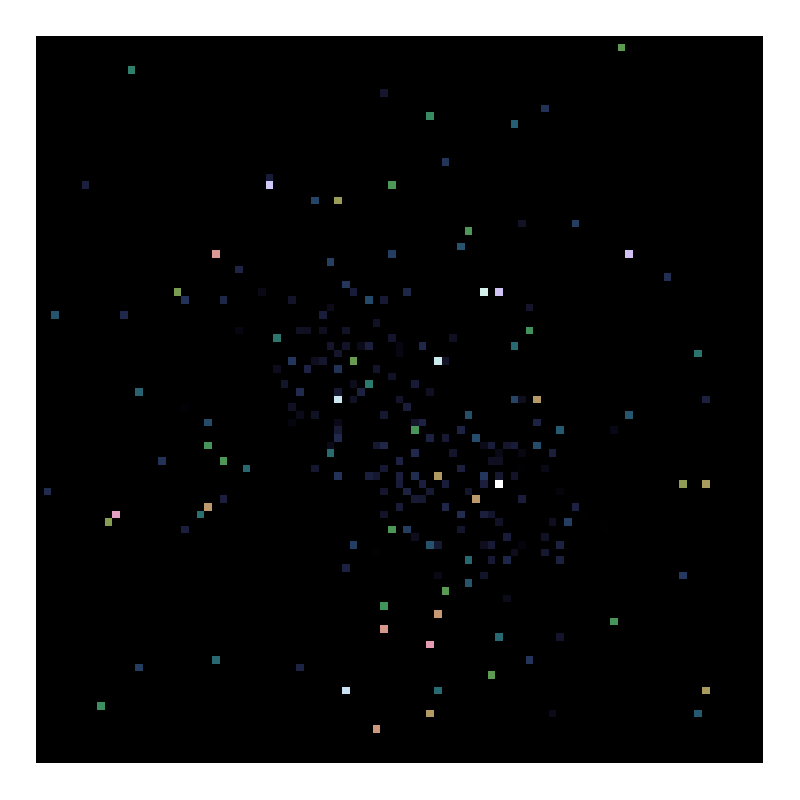
\includegraphics[width=1.00\linewidth, clip, trim= 0.25in 0.25in 0.25in 0.25in]{./chapters/05.pcdm/randomProblem/random_1k_block1.png}
		\caption{8k iterations}
		\label{pcdm:adaption:randomProblem:block11}
	\end{subfigure}
	\begin{subfigure}[b]{0.245\linewidth}
		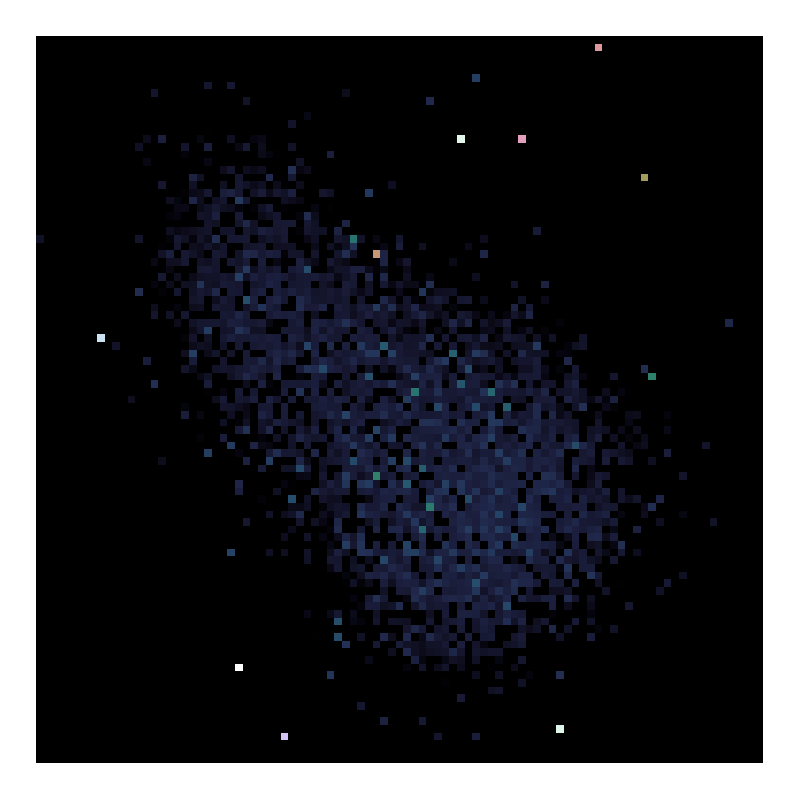
\includegraphics[width=1.00\linewidth, clip, trim= 0.25in 0.25in 0.25in 0.25in]{./chapters/05.pcdm/randomProblem/random_10k_block1.png}
		\caption{80k iterations}
		\label{pcdm:adaption:randomProblem:block12}
	\end{subfigure}
		\begin{subfigure}[b]{0.245\linewidth}
		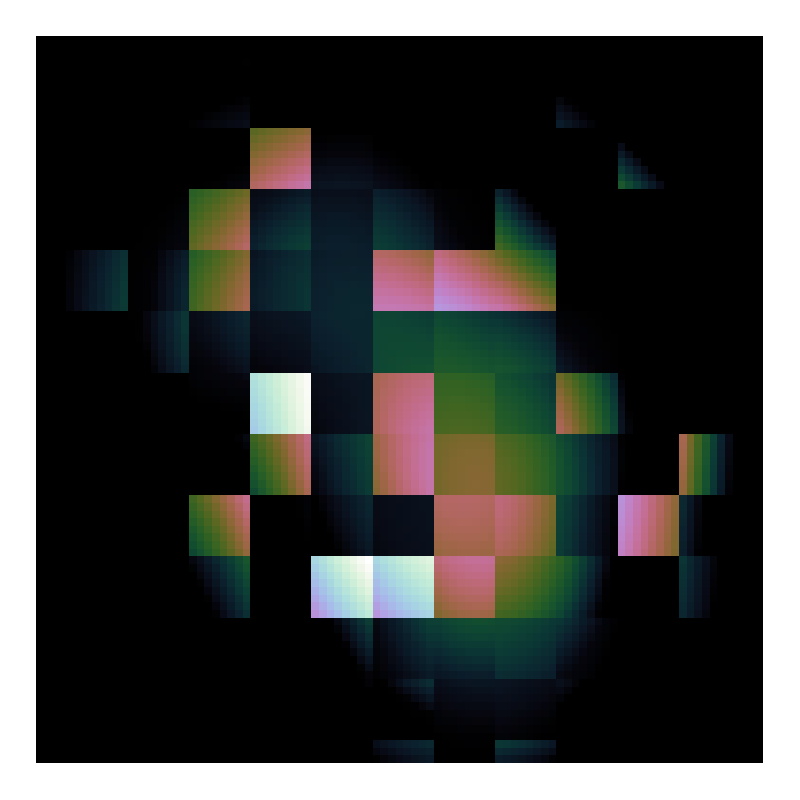
\includegraphics[width=1.00\linewidth, clip, trim= 0.25in 0.25in 0.25in 0.25in]{./chapters/05.pcdm/randomProblem/random_1k_block8.png}
		\caption{8k iterations, $8^2$ block}
		\label{pcdm:adaption:randomProblem:block81}
	\end{subfigure}
		\begin{subfigure}[b]{0.2405\linewidth}
		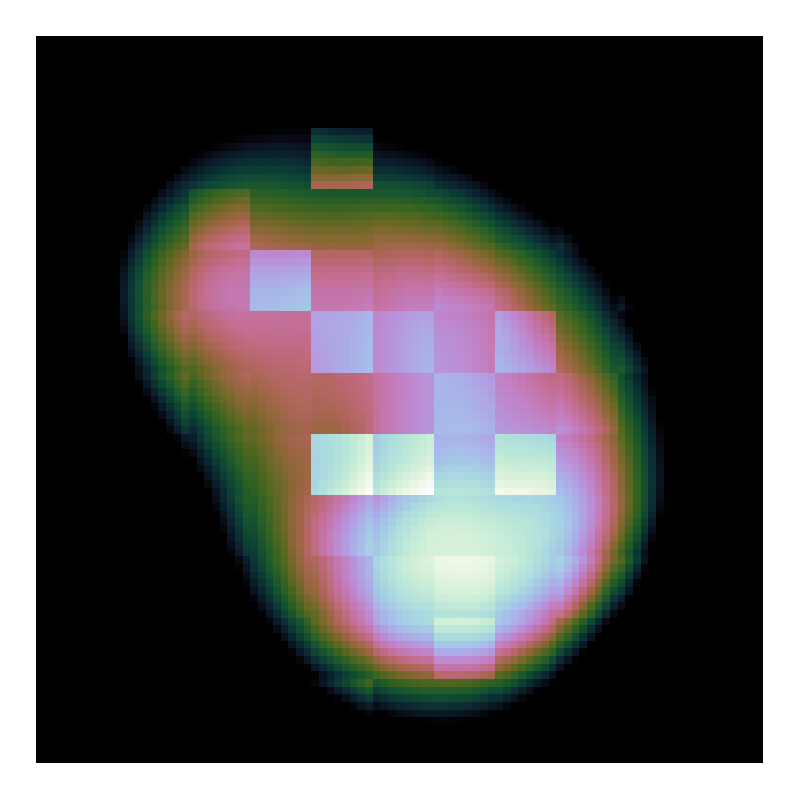
\includegraphics[width=1.00\linewidth, clip, trim= 0.25in 0.25in 0.25in 0.25in]{./chapters/05.pcdm/randomProblem/random_10k_block8.png}
		\caption{80k iterations, $8^2$ block}
		\label{pcdm:adaption:randomProblem:block82}
	\end{subfigure}
	\caption{Random parallel deconvolutions on the LMC N132D supernova remnant.}
	\label{pcdm:adaption:randomProblem}
\end{figure}

The Figure \ref{pcdm:adaption:randomProblem} shows the behaviour on the LMC observation. The reconstructions receive obvious artifacts from the random selection strategy. The blocks, which get selected in the first few iterations, keep their over-estimated values. The parallel algorithm needs to select them several times to reduce their value. That is why even after 80k iterations, the N132D supernova remnant gets only hinted at in Figure \ref{pcdm:adaption:randomProblem:block12}. Until the over-estimated blocks get selected again, the algorithm cannot do useful updates in that region.

This behavior is pronounced when we choose a block size of one pixel (i.e. we do not group pixels into blocks). A naive solution is to increase the block size. This leads to fewer possible blocks in the image, and obviously an increased chance to select the same block again in later iterations. But as we see in Figure \ref{pcdm:adaption:randomProblem:block82}, the same problem exists with larger block sizes, although less pronounced. After 80k iterations the N132D supernova remnant is visible, but a few random blocks still contain too much of the emission in that area.

A random selection strategy needs a prohibitive large number of iterations to converge. But we cannot simply switch out the selection strategy. The random selection strategy is at the core of the Parallel coordinate descent methods. Remember the ESO arises from the fact that we select $tau$ pixels uniformly at random. When we select $\tau$-pixels with a greedy strategy, we might break the ESO, and the parallel algorithm may not converge at all.

To solve this behavior, we introduce the pseudo-random selection strategy:  We select a block at random, but greedily search in the neighborhood for the optimal block to optimize. The size of the neighborhood can be defined by the user. It is essentially a mix between a greedy and a random selection strategy. If we choose the neighborhood to be the whole image, we arrive at a greedy strategy. If we choose the neighborhood to be just one block, we are back at a random strategy. The mixture of the greedy and random strategy allows us to fix the problems with the pure random strategy, without breaking any assumptions from the Parallel Coordinate Descent Method's ESO. The mixture of the greedy and random strategy is represented in a 'Search Fraction' parameter. It is a tuning parameter of our parallel coordinate descent algorithm. The optimal value for the Search Fraction is explored later in Section \ref{pcdm:results:fraction}. We now introduce three related extensions, which speed up the  parallel coordinate descent in practice: An active set heuristic, Restarting heuristic and a 'Minor' cycle.




